\documentclass[a4paper,oneside,10pt]{article}
\usepackage{wallpaper}
\usepackage{float}
\usepackage[utf8]{inputenc}
\usepackage[T1]{fontenc}
\usepackage{circuitikz}
\usepackage{amsmath}
\usepackage{graphicx}
\usepackage{booktabs}
\usepackage{listings}
\usepackage{xcolor}
\usepackage{hyperref}

\setlength{\textwidth}{16cm} %
\setlength{\textheight}{23cm} %
\setlength{\oddsidemargin}{0cm} %
\setlength{\evensidemargin}{0cm} %
\setlength{\topmargin}{0cm}

\CenterWallPaper{1.01}{bg.pdf}

\hypersetup{colorlinks=true,urlcolor=blue,linkcolor=black}

\lstset{
  language=Python,
  basicstyle=\ttfamily\scriptsize,
  keywordstyle=\color{blue},
  commentstyle=\color{gray},
  stringstyle=\color{red!60!black},
  numbers=left,
  numberstyle=\tiny\color{gray},
  frame=single,
  breaklines=true,
  showstringspaces=false,
  tabsize=4,
  extendedchars=true,
  literate=
    {á}{{\'a}}1 {à}{{\`a}}1 {â}{{\^a}}1 {ã}{{\~a}}1
    {é}{{\'e}}1 {ê}{{\^e}}1 {í}{{\'i}}1
    {ó}{{\'o}}1 {ô}{{\^o}}1 {õ}{{\~o}}1
    {ú}{{\'u}}1 {ç}{{\c c}}1
    {Á}{{\'A}}1 {É}{{\'E}}1 {Í}{{\'I}}1 {Ó}{{\'O}}1 {Ú}{{\'U}}1 {Ç}{{\c C}}1
}

\begin{document}

\noindent Lista de Exercícios: Método de Gauss--Seidel para Sistemas Lineares. \\
Cálculo Numérico (Integral)\\
Profa Raquel Lobosco\\
2026.2\\
\\
\textbf{EQUIPE:} Leonardo Tomasela Leal \quad RA: 170291 \\

\section{Sistema Linear}
Considere o sistema
\[
\begin{cases}
10x - y + 2z = 6,\\
-x + 11y - z = 22,\\
2x - y + 10z = -10.
\end{cases}
\]

\section{Parte Manuscrita (Itens 1 a 4)}

\subsection{Item 1: Forma matricial}
\begin{figure}[H]
\centering
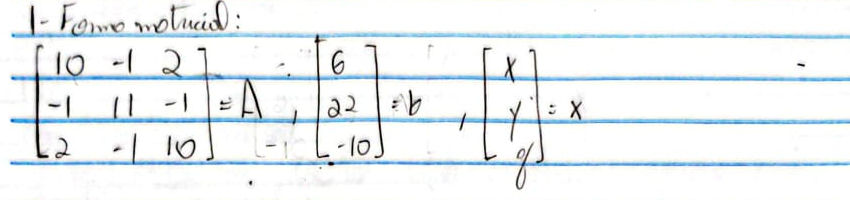
\includegraphics[width=0.95\textwidth]{item1.png}
\end{figure}

\subsection{Item 2: Dominância diagonal por linhas}
\begin{figure}[H]
\centering
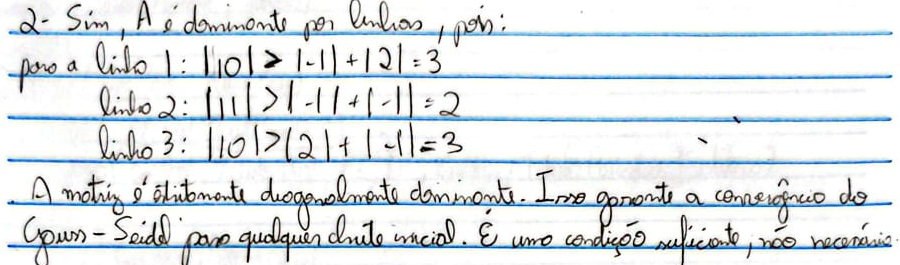
\includegraphics[width=0.95\textwidth]{item2.png}
\end{figure}

\subsection{Item 3: Fórmulas iterativas de Gauss--Seidel}
\begin{figure}[H]
\centering
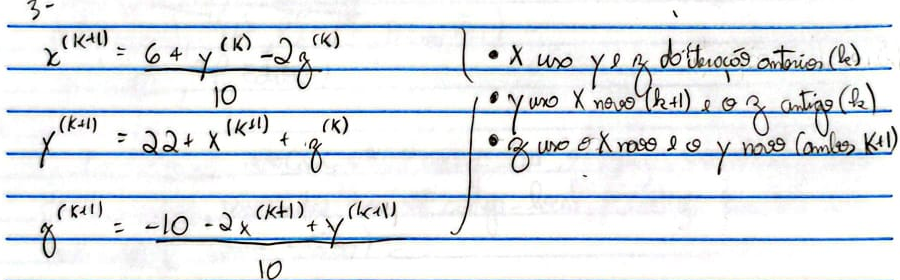
\includegraphics[width=0.95\textwidth]{item3.png}
\end{figure}

\subsection{Item 4: Três primeiras iterações com $x^{(0)}=(0,0,0)$}
\begin{figure}[H]
\centering
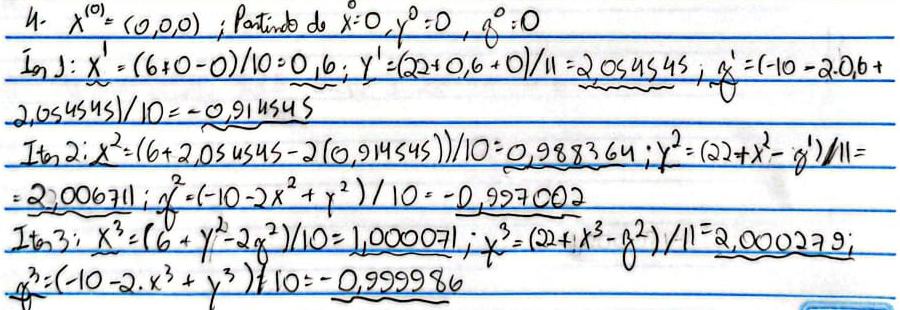
\includegraphics[width=0.95\textwidth]{item4.png}
\end{figure}

\section{Parte Computacional (Itens 5 a 7)}

\subsection{Item 5: Implementação em Python}
O código a seguir implementa o método de Gauss--Seidel com critério de parada
$\|x^{(k)}-x^{(k-1)}\|_\infty < 10^{-5}$.

\lstinputlisting{gauss_seidel_corrigido.py}

\medskip
\noindent\textbf{Número de iterações:} 6.\\
\textbf{Solução aproximada obtida:} $x \approx 1{,}000000$, \ $y \approx 2{,}000000$, \ $z \approx -1{,}000000$.

\subsection{Item 6: Tabela das iterações}
\begin{table}[H]
\centering
\begin{tabular}{rcccc}
\toprule
$k$ & $x^{(k)}$ & $y^{(k)}$ & $z^{(k)}$ & $\|x^{(k)}-x^{(k-1)}\|_\infty$ \\
\midrule
1 & 0.600000 & 2.054545 & -0.914545 & $2.0545\times10^{0}$ \\
2 & 0.988364 & 2.006711 & -0.997002 & $3.8836\times10^{-1}$ \\
3 & 1.000071 & 2.000279 & -0.999986 & $1.1708\times10^{-2}$ \\
4 & 1.000025 & 2.000004 & -1.000005 & $2.7554\times10^{-4}$ \\
5 & 1.000001 & 2.000000 & -1.000000 & $2.3892\times10^{-5}$ \\
6 & 1.000000 & 2.000000 & -1.000000 & $1.2626\times10^{-6}$ \\
\bottomrule
\end{tabular}
\end{table}

\subsection{Item 7: Gráficos}
\begin{figure}[H]
\centering
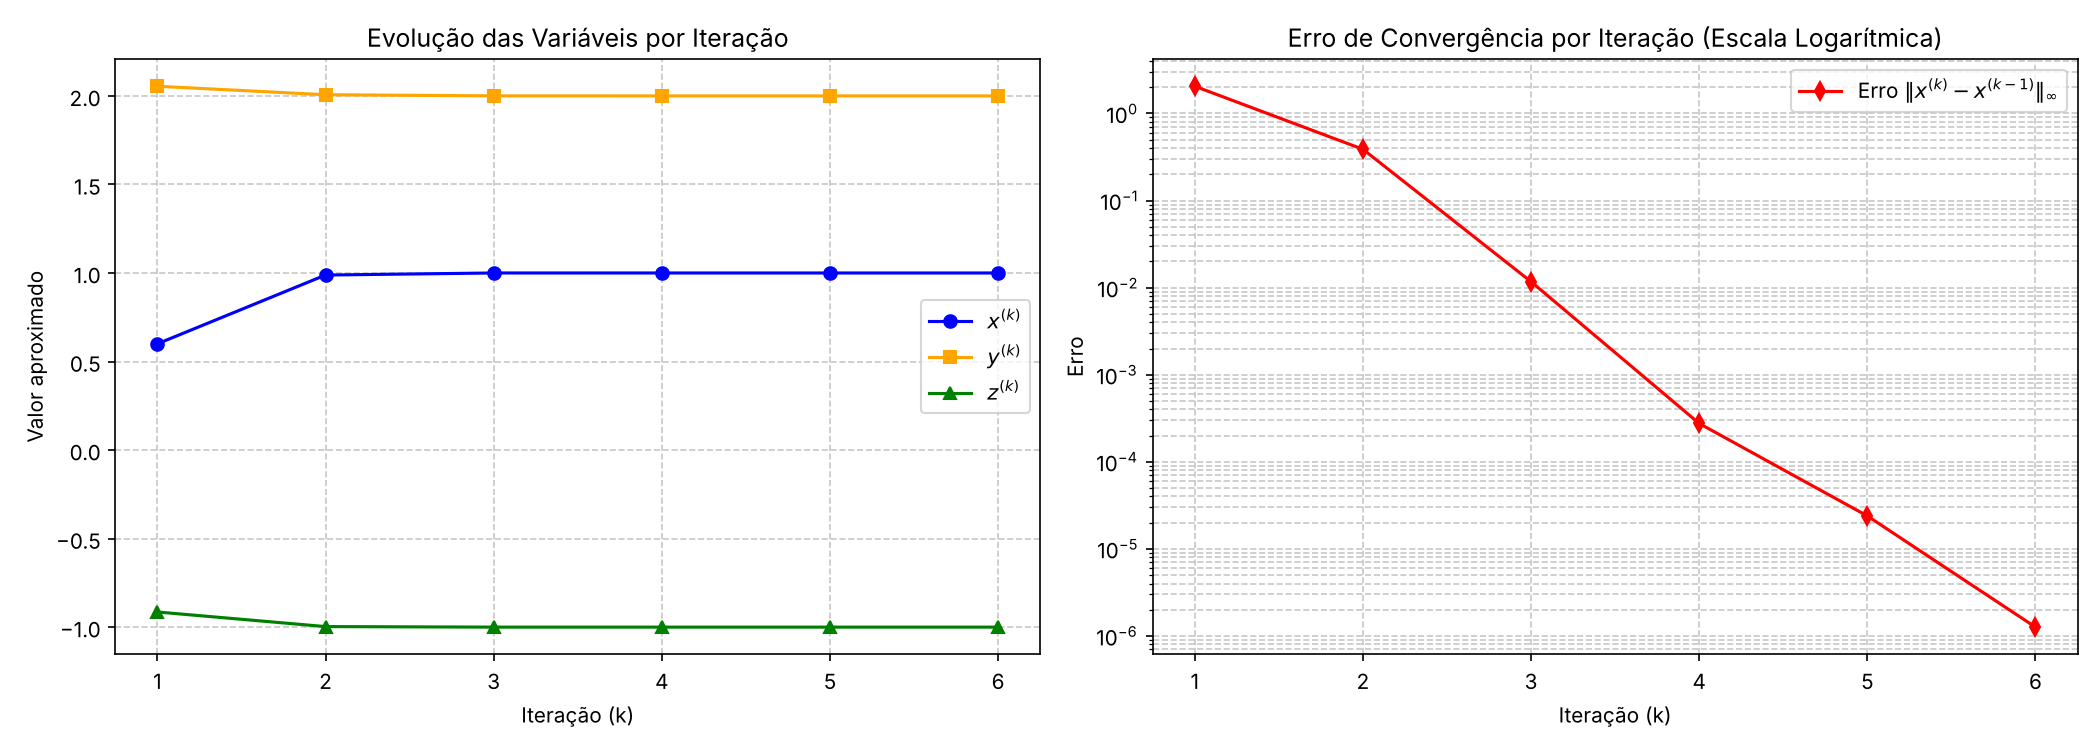
\includegraphics[width=\textwidth]{graficos_gauss_seidel.png}
\end{figure}

\noindent (a) À esquerda: $x^{(k)}$, $y^{(k)}$ e $z^{(k)}$ em função de $k$. \\
(b) À direita: erro entre iterações, $\|x^{(k)}-x^{(k-1)}\|_\infty$, em função de $k$, em escala logarítmica.

\section{Anexos}

Código no Google Colab: \url{https://github.com/leonardo2004/Calculo-Numerico/blob/main/Sistemas%20lineares%202/Sistemas_linerares_em_c%C3%A1lculo_num%C3%A9rico.ipynb}

\end{document}
